\documentclass {CSEThesis}
% Standard packages
\usepackage{amsmath}        % Extra math definitions
\usepackage{graphics}       % PostScript figures
\usepackage{setspace}       % 1.5 spacing
%\usepackage{psfig,epsfig}
\usepackage{multicol}
% \usepackage{subfigure}
\usepackage{epsfig,color}
\setlength{\parindent}{0in}
\setlength{\parskip}{\baselineskip}
\setlength{\textheight}{9in}
\setlength{\textwidth}{6in}
\setlength{\topmargin}{0in}
\setlength{\evensidemargin}{0in}
\setlength{\oddsidemargin}{0in}
\usepackage{tikz}
\usepackage{subcaption}
\usepackage{scalefnt}
\usepackage{booktabs}
\usepackage[margin=1in, headsep=10pt, footskip=24pt]{geometry}
\usepackage{titlesec}

\nocite{GoogleDriveRegion}
\nocite{GoogleDriveExperiments}
% \usepackage{amsmath,amsfonts,amsthm,enumerate,amssymb}
\usepackage{url}
\usepackage{hyperref}
% Custom packages
%\usepackage[first]{datestamp}   % Datestamp on first page of each chapter
\usepackage[style = apa]{biblatex}
\addbibresource{btp.bib}

\usepackage{color}
\usepackage{colortbl} % Enables row coloring
\usepackage{xcolor}   % Provides color definitions
\usepackage{wrapfig}
\usepackage{float}
%===== page layout
% Define the side margins for a right-side page
%\insidemargin = 1.3in \outsidemargin = 0.9in
% Above margin is space above the header
% Below margin is space below footer
%\abovemargin = 1.5in \belowmargin = 0.05in
\usepackage{etoolbox}
\makeatletter
\patchcmd{\tableofcontents}{\@starttoc{toc}}{\vspace*{-2cm}\@starttoc{toc}}{}{}
\makeatother


\makeatletter
\def\@makechapterhead#1{%
  \vspace*{-20pt}
  {\parindent \z@ \raggedright \reset@font
    \Huge\bfseries #1\par\nobreak
    \vskip 20pt
  }}
\makeatother


\btptitle = {Auditing Depression Prediction Automated Decision System} % { and } are needed around your name
\name = { \makebox[3cm]{Judy Yang} \hspace{2cm} \makebox[3cm]{Era Sarda} \\  
    \vspace{1mm} \makebox[3cm]{\texttt{hy1331@nyu.edu}} \hspace{2cm} \makebox[3cm]{\texttt{es6790@nyu.edu}}}         
\guide = {Instructors\\Prof. Emily Black and Lucas Rosenblatt}


\begin{document}

\begin{titlepage}
\begin{center}
\textheight 15.5in \textwidth 12.5in {\large\sf  \textbf{\the\btptitle}}\\[12ex]
{\small{\textsl{ \textbf{Final Project Report Submitted \\
in Partial Fulfillment of the Requirements \\
for the course
\\[1ex]\small \bf DS-GA 1017 Responsible Data Science}}}}\\[7ex] \emph{by} \\
[4ex]{\sf \textbf{\the\name}\\
[1ex]
\emph{under the guidance of}\\[2ex]
{\sf \bf \the\guide} \\[7ex]

\vspace{1.2in}

 \begin{figure}[!h]
 \hfill
 
\psfig{file=nyulogo.png,width=0.10\textwidth} \hfill \
 \end{figure}

{\sl \bf{to the}} \\[1ex]

{\small\bf CENTER FOR DATA SCIENCE}  \\[1ex]
{\small \bf{NEW YORK UNIVERSITY \\NEW YORK - 10012, NY}}
%\\[2ex]
%
%  {\color{red} \hrule height 0.5ex}
% \vskip 1ex
% May \the\year 
\end{center}
\end{titlepage}

\newpage
\chapter*{\centering Abstract}
\textit{\quad 
This report presents a fairness audit of a high-performing ensemble machine learning model developed for depression prediction, originally designed for a Kaggle competition using synthetic mental health data. While the model achieves high predictive accuracy by combining AdaBoost, CatBoost, XGBoost, Logistic Regression, and LGBMClassifier, our audit reveals critical disparities in subgroup performance. Through detailed analysis of feature correlations, missing data patterns, and regional representation, we identify structural and cultural biases in the dataset, particularly affecting employment status and age subgroups. Stakeholder perspectives (patients, families, professionals, and institutions) are also mapped to understand real-world implications. Fairness evaluations using Fairlearn’s MetricFrame and ThresholdOptimizer expose significant performance gaps: students experience high false positive rates, while working professionals face high false negative rates. Post-processing mitigation with equalized odds constraints reduces these disparities, though at a cost to overall accuracy. LIME is further applied to interpret individual predictions, uncovering group-specific reasoning patterns. This audit highlights the need for fairness-aware evaluation, culturally grounded feature design, and subgroup-specific calibration when deploying automated decision systems in high-stakes domains like mental health.
}


\tableofcontents 
\pagenumbering{arabic}
\def\headrulehook{\color{black}}      % Color the header rule

%========== Chapters
\typeout{}
\chapter{Background}
\pagenumbering{arabic}\hspace{3mm}

Depression and other mental illnesses have long been known to exhibit significant gender disparities in their reported prevalence \parencite{astbury1999gender}. In the case of depression — including both depressive symptoms and Major Depressive Disorder (MDD) — research in the United States has shown that “females experience 1.5- to 3-fold higher rates than males beginning in early adolescence” \parencite[p. 165]{APA2013DSM5}. However, studies have also found that this gender gap is considerably smaller in many developing countries \parencite{Sartorius1983}. This discrepancy raises the question of whether systematic biases—such as those introduced through data collection methods (e.g., census formats) or through Western gender norms and stereotypes—may be contributing to the observed differences in depression prevalence.

Despite this possibility, the gender disparity in depression has often been accepted as fact within the field of clinical psychology and embedded into the “gold standard” of psychiatric diagnosis, the \textit{Diagnostic and Statistical Manual of Mental Disorders, Fifth Edition} (DSM-5) \parencite{huntExploringGoldStandardEvidence2018}. Given these potential underlying biases in how mental health data is framed and interpreted, it is reasonable to expect that machine learning (ML) models trained to predict depression may also exhibit gender-based biases.

In this project, we propose to audit a high-performing ML model developed by Mahdi Ravaghi \parencite{ravaghiS04E11MentalHealth2024}, which won first place in Season 4, Episode 11 of Kaggle’s \href{https://www.kaggle.com/competitions/playground-series-s4e11}{Playground Series Competition}, titled \textit{Exploring Mental Health Data} \parencite{playground-series-s4e11}. The competition tasked participants with predicting mental health outcomes using a structured dataset, and submissions were evaluated solely based on accuracy. Ravaghi’s ensemble-based model achieved the highest accuracy among more than 2,500 submissions.

To evaluate both the performance and fairness of this model, we conducted a series of post hoc analyses including accuracy benchmarking, group-specific fairness metrics, and model interpretability techniques. We used Fairlearn’s \texttt{MetricFrame} to assess disparities in predictive outcomes across sensitive groups, applied post-processing mitigation through threshold optimization to address identified inequities, and used LIME (Local Interpretable Model-agnostic Explanations) \parencite{ribeiro2016why} to interpret how feature contributions vary at the individual level. While gender was our initial focus as the sensitive attribute, exploratory analysis led us to shift attention to employment status — specifically, whether individuals were working professionals or students — as this distinction revealed more pronounced disparities in model performance. Together, these methods aim to reveal not only how well the model performs, but also whom it serves—and whom it may potentially overlook or misclassify.

% \cleardoublepage 
\typeout{}
\chapter{About the Dataset}

The dataset used in the Kaggle competition \parencite{raoDepressionSurveyDataset} includes a range of predictors relevant to mental health. For the purposes of our fairness audit, we consider \texttt{Gender} as the primary sensitive attribute. In addition to gender, features such as profession, degree, and dietary habits may act as proxy variables, potentially capturing implicit gender-related signals.

Beyond individual attributes, the model’s performance may also be influenced by geographic and cultural biases embedded in the dataset. The data originates from the Indian subcontinent, but distribution plots
[\href{https://colab.research.google.com/drive/1V5NlYPUzOfSxUoDHg67yVfatMXSTWNSU?usp=sharing}{1}, \href{https://www.google.com/maps/d/edit?mid=17YtHn2h6j22KFGfMiAvcx5rToAd4Ukw&usp=sharing}{2}] suggest it is disproportionately sampled from major urban centers in North and Central-West India. Areas such as smaller cities, rural regions, and the South, Central-East, and North-East are notably underrepresented. This sampling imbalance raises concerns about whether the dataset reflects the full regional diversity of India, and whether the trained model can generalize well across culturally and geographically distinct populations.

Importantly, the dataset is \textbf{synthetically generated}. As a result, biases in regional distribution may stem from (i) the original data used for synthesis, (ii) the design of the generation algorithm, or (iii) deliberate sampling decisions. Yet, there appears to be no clear rationale for the selection of included cities. The sampled regions do not consistently correspond to city size, population density, state capitals, metropolitan zones, or any coherent regional grouping. This absence of justification limits confidence in the model’s representativeness and generalizability.

Furthermore, the dataset omits important cultural and familial dimensions that are particularly salient in the Indian context. In many Asian societies, family structure, interdependence, and relationship quality play central roles in shaping psychological well-being. For instance, Lu and colleagues \parencite{lu2010understanding} demonstrate that even the conceptualization of depression differs significantly between Chinese and American populations, reinforcing the importance of culture in mental health modeling.

To that end, variables capturing intergenerational living, number of dependents, or relationship satisfaction would have been valuable additions to the dataset. Their inclusion could offer more culturally grounded insights into depression risk, especially for a demographically diverse population like India’s. Without these features, the model may overlook key factors that contribute to mental health outcomes in the region.

See Appendix~\ref{appendix} for further details on data distribution and regional representation.
% \cleardoublepage 
\typeout{}
\chapter{Implementation and Validation}

This section presents our understanding of the implementation of the depression prediction model developed for the Kaggle Playground Series S4E11 competition. The code was written by Mahdi Ravaghi and publicly released as the winning solution. Our goal here is to demonstrate a high-level understanding of how the system operates, how the data was processed, and how the model was validated for its stated objective of maximizing predictive accuracy.

\section{Data Cleaning and Pre-processing}

The original pipeline involved substantial pre-processing to prepare the dataset for machine learning. Categorical features were cast as \texttt{category} dtype, with category alignment enforced across the training and test datasets. For certain models (e.g., AdaBoost and XGBoost), ordinal encoding was applied to categorical variables. Continuous features with missing values were imputed using mean imputation. The final feature matrix was standardized for models that were sensitive to feature scaling (e.g., Logistic Regression and Ridge Regression). Importantly, gender and other categorical fields were preserved as-is to allow downstream auditing of subgroup behavior. The data itself is synthetic, generated from an undisclosed private dataset, and does not include real personal identifiers.

\section{High-level Implementation of the System}

The system follows a stacked ensemble architecture. The first layer (L1) consists of five base models: AdaBoost, CatBoost, XGBoost, LightGBM, and Logistic Regression. Each of these models was trained independently and generated probability outputs on the validation set. These predictions were passed to a second-level ensemble (L2), where two models—Logistic Regression and Ridge Regression—were trained using the logit-transformed probabilities of the base models as inputs. These L2 models effectively learned how to weight the base model predictions. Finally, an L3 ensemble combined the outputs of the L2 models using a weighted average, with the optimal weights learned via hyperparameter tuning (using Optuna). This layered design was intended to maximize accuracy while leveraging the strengths of diverse classifiers.

The original implementation used stratified $k$-fold cross-validation to evaluate model performance and select hyperparameters. This approach is standard in ML competitions and helps ensure robust performance estimates by averaging accuracy across multiple validation splits.

\section{Validation and Alignment with Stated Goals}

The ADS was validated using stratified cross-validation, and the stated goal—maximizing accuracy—was achieved, with the final model reaching approximately 94–96\% average accuracy across folds. However, since the competition’s test set did not contain ground-truth labels, external validation and fairness analysis were not originally conducted. To audit the model for fairness, we created a fixed train-validation split from the training data. This enabled the use of fairness metrics such as selection rate, true/false positive rates, and enabled consistent subgroup analysis via Fairlearn’s \texttt{MetricFrame}.

We also discovered that cross-validation introduces variability in subgroup representation across folds, complicating fairness analysis. A fixed validation set allowed for reproducible and interpretable group-level metrics. Figure~\ref{fig:model_before} shows model performance under cross-validation, and Figure~\ref{fig:model_after} shows performance under our fixed split.

\begin{figure}[H]
\centering
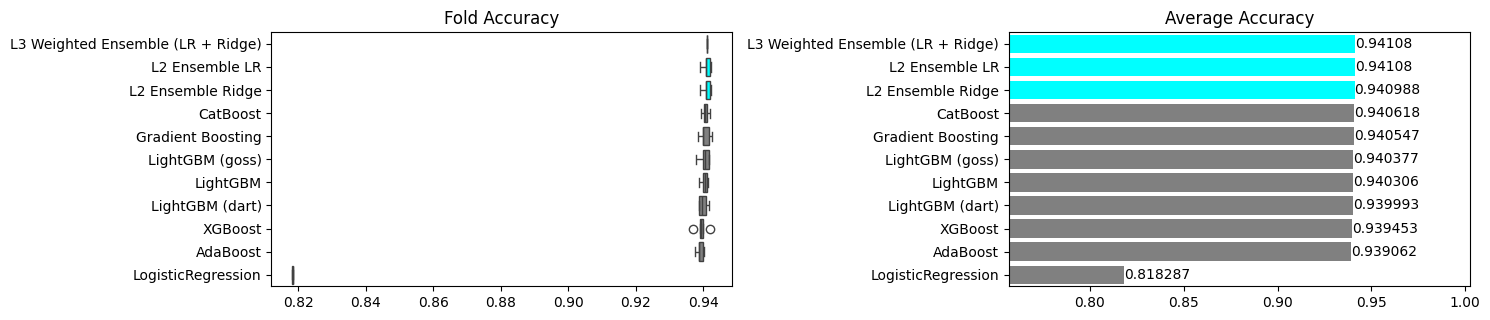
\includegraphics[width=0.87\linewidth]{figures/model_before.png}
\caption{Cross-validated accuracy comparison of different models under the original ensemble pipeline. The L3 weighted ensemble achieves the highest mean accuracy.}
\label{fig:model_before}
\end{figure}

\begin{figure}[H]
\centering
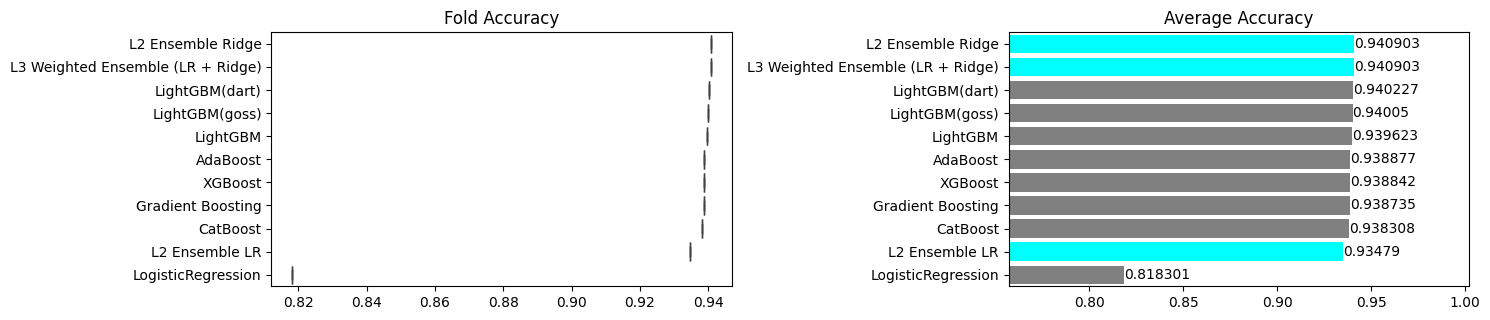
\includegraphics[width=0.87\linewidth]{figures/model_after.png}
\caption{Accuracy comparison of models using a fixed train-validation split. Overall rankings remain consistent, but this approach enables fair and consistent subgroup evaluation.}
\label{fig:model_after}
\end{figure}

That said, our fixed-split strategy may have introduced information leakage or artifacts, as the data is synthetic and its generative process is not fully disclosed. Future work could involve generating privacy-preserving synthetic datasets using differentially private mechanisms or correlation-aware generative models.\\
In summary, the implementation was accurate and sophisticated in terms of ensemble architecture and optimization, but fairness and robustness to distributional shift were not considered in the original validation pipeline. Our re-validation using a fixed split enabled a more thorough fairness audit aligned with the needs of a real-world ADS.
% \cleardoublepage 
\typeout{}
\chapter{Audit Outcomes}

% Note: Since we don't have access to true labels of original test set of the Kaggle Competition, we split the original training data into train and test data (4:1 ratio) for validating the model performance across various audit tests. The results we obtained may or may not be highly accurate, since train-test split might have caused information leakage. \\
% (maybe try to generate dp synthetic dataset using the "final depression dataset" in correlated mode to once check the model performance generalization???) 



% 1. dropping name and city has no significant affect on accuracy of the model.\\
% 2. for 2 submodels gb and adb, numerical value columns were imputed with mean values - [Academic Pressure, Work Pressure, CGPA, Study Satisfaction,Job Satisfaction] - this seems unjustifiable, since imputing mean of academic pressure value to a professional, or work pressure value to a student doesn't make sense. Yet, when model was run for these 2 categories seperately, with dropping the non-relevant columns, the metrics obtained were quite similar to what was obtained before, implying the model's robustness, which can be explained by the usage of ensembling several models \parencite{black2021selective}. The FPR  and FNR parity genderwise ia high, however, w.r.t. employment status, working professionals have high FNR and students have high FPR. \\
% (-- have to look into 'Profession' and 'CGPA' for this. And lime values too. )\\
% checked lime values for 10 false positive classifications--pattern?\\
% top 5 points for explanations suggest ---\\


\section{Experiments}
Initial experiments showed that dropping the \texttt{Name} and \texttt{City} features from the dataset had no significant impact on the model’s overall accuracy as well as other metrics like FNR/FPR and fairness metrics as can be seen in Figure~\ref{fig:orig_vs_drop}. This suggests that these features did not carry meaningful predictive information and that the model is not overly reliant on potentially privacy-sensitive attributes. Other relevant results w.r.t. overall and genderwise FNR/FPR/Selection Rate Difference are included in Appendix~\ref{feature_corr} (Figures~\ref{fig:region_overall},~\ref{fig:region_gender}). 

\begin{figure}[H]
    \centering
    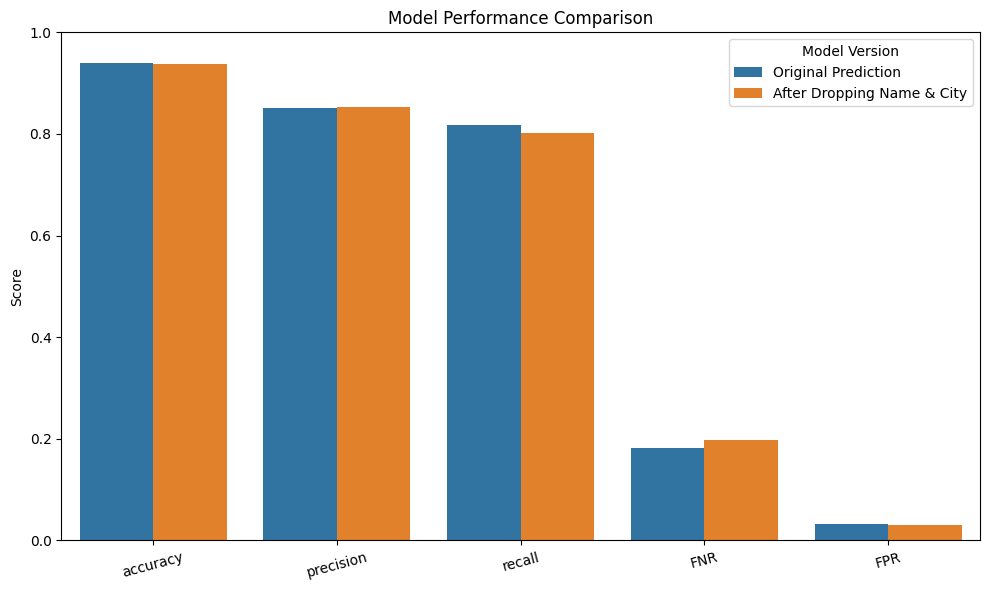
\includegraphics[width=0.6\linewidth]{figures/orig_vs_drop.png}
    \caption{Results before and after dropping sensitive features}
    \label{fig:orig_vs_drop}
\end{figure}

An interesting observation emerged from examining how the two sub-models : Gradient Boosting (GB) and AdaBoost (ADB) handled missing data. These models imputed missing values in numerical columns such as \texttt{Academic Pressure}, \texttt{Work Pressure}, \texttt{CGPA}, \texttt{Study Satisfaction}, and \texttt{Job Satisfaction} using mean imputation. While this method is common, it can be problematic in our context. For example, imputing the average academic pressure of students for a working professional lacks contextual validity, and vice versa. Yet, when the ensemble model was retrained and evaluated separately for students and working professionals (after dropping the irrelevant features for each group), the resulting performance metrics were close to the original scores (Figure~\ref{fig:orig_vs_stu}). This implies a degree of robustness in the overall ensemble model architecture, likely due to the averaging effects of combining multiple learners \parencite{black2021selective}. However, another observation to note here was that the outputs of weighted probabilities of the ensemble model go out of the range of [0,1] for various datapoints of working professional group specifically. The unbounded outputs are due to the application of Ridge and Logistic regression on base models' probabilites, suggesting the need for post-hoc calibration (See figure~\ref{fig:prob_distri} in Appendix~\ref{post_train}). Although such changes are beyond the scope of this audit, we recommend applying sigmoid transformation or calibration techniques like Platt scaling to ensure the outputs conform to probabilistic interpretations. 


\begin{figure}[h]
    \begin{minipage}{0.49\textwidth}
        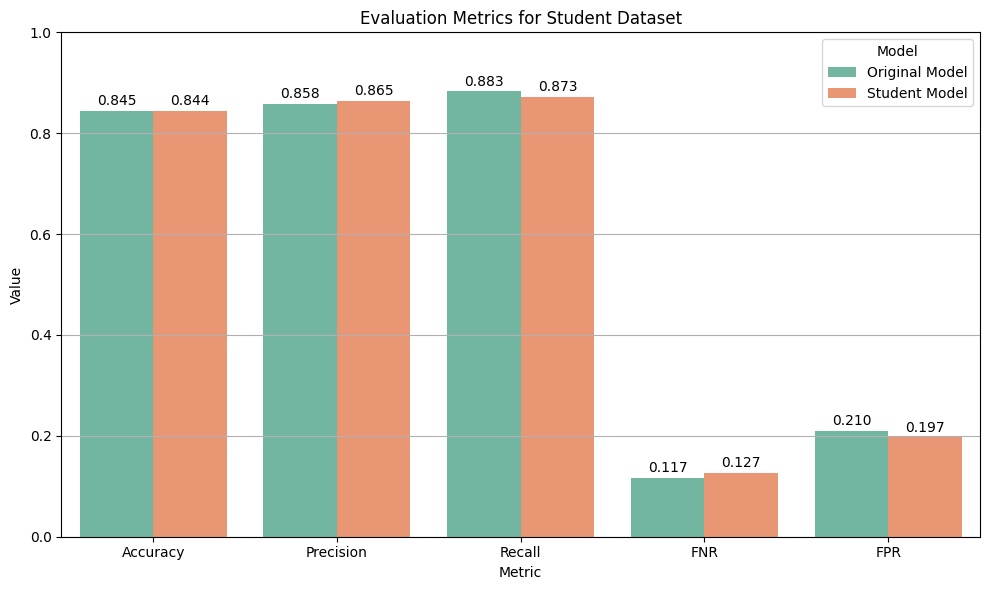
\includegraphics[width=\linewidth]{figures/orig_vs_stu.png} 
    \end{minipage}
    \hfill
   \begin{minipage}{0.49\textwidth}
        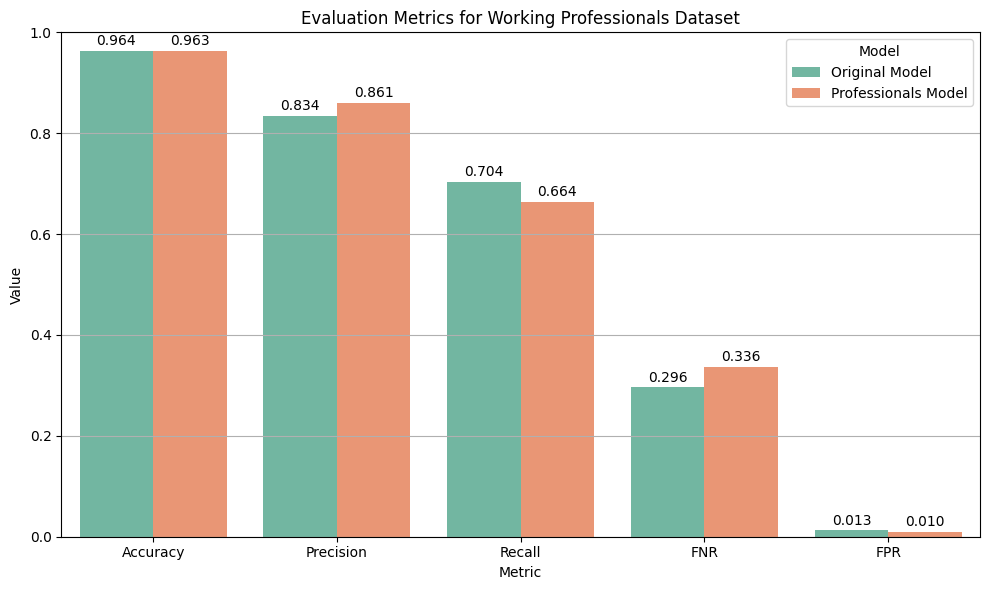
\includegraphics[width=\linewidth]{figures/orig_vs_prof.png} 
    \end{minipage}
    \caption{Metrics Comparison before and after dropping non-relevant features for Students and Working Professionals}
    \label{fig:orig_vs_stu}
\end{figure}

\section{Model Fairness}

To evaluate the fairness of our model, we passed its predictions into \texttt{Fairlearn}’s \texttt{MetricFrame}, using \texttt{Gender} as the sensitive feature. This allowed us to measure not only overall accuracy but also group-specific metrics such as selection rate, false positive rate (FPR), and true positive rate (TPR). These metrics were chosen because they reflect how differently the model behaves across demographic groups in ways that affect real-world outcomes. For example, TPR captures whether the model consistently identifies depression when it is truly present, while FPR reflects the cost of wrongly flagging individuals as depressed. Selection rate offers a lens into how often each group is predicted as positive, regardless of correctness—highlighting disparities in model attention or prioritization. These group-wise metrics provide a more granular understanding of equity than accuracy alone, especially in high-stakes contexts like mental health screening. Contrary to our initial expectations, the model exhibited minimal disparity across gender groups.

\begin{figure}[h]
    \centering
    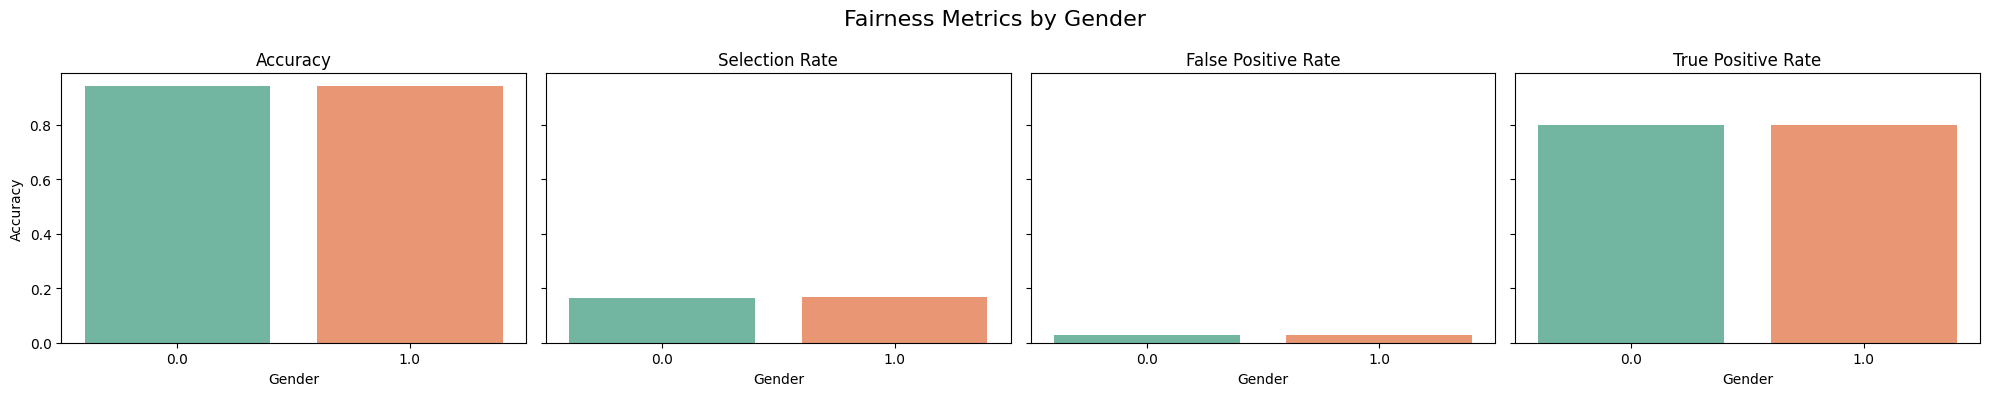
\includegraphics[width=\linewidth]{figures/mf_gender.png}
    \caption{Fairness metrics of the model, with Gender as the sensitive feature.}
    \label{fig:mf_gender}
\end{figure}

As shown in Figure~\ref{fig:mf_gender}, both male and female groups achieve comparable accuracy, selection rate, and error rates. These results suggest that the model is \textit{not} exhibiting strong gender-based bias in its predictions, despite broader societal patterns that might suggest otherwise.

To further validate this finding, we examined fairness across subgroups defined by both \texttt{Gender} and employment status (student or working professional). Once again, we observed no meaningful disparities, as illustrated in Figure~\ref{fig:gender_stu_prof}.

\begin{figure}[h]
    \centering
    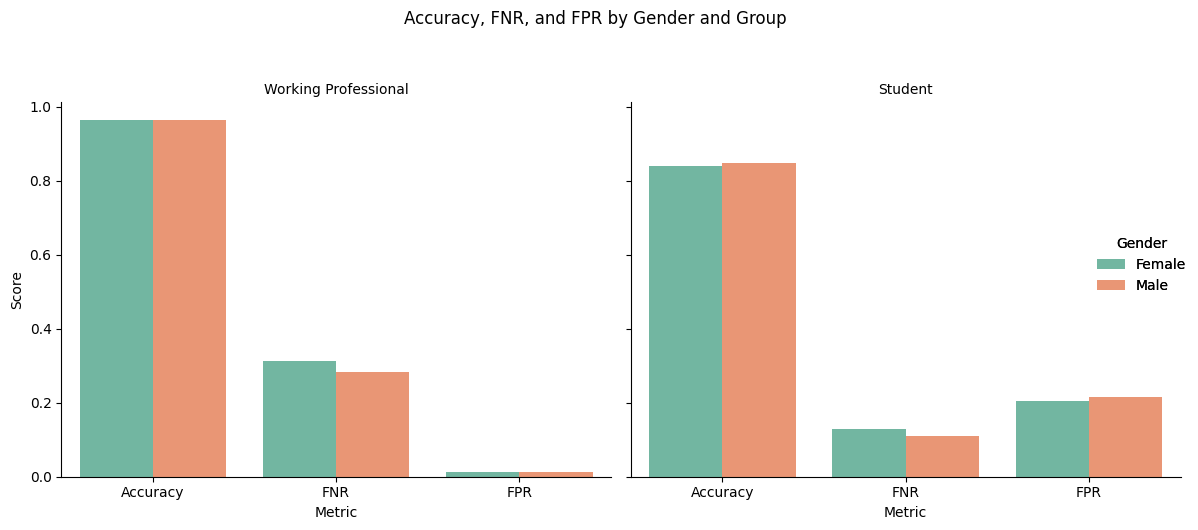
\includegraphics[width=\linewidth]{figures/gender_stu_prof.png}
    \caption{Fairness metrics of the model across employment subgroups, with Gender as the sensitive feature.}
    \label{fig:gender_stu_prof}
\end{figure}

Given the lack of observed gender disparity, we decided to explore alternative sensitive features. Our choice to use \texttt{Working Professional or Student} status as the next axis of analysis was guided by our initial exploratory data analysis. There, we uncovered a strong relationship between age and depression, with younger individuals — particularly students — exhibiting significantly higher depression rates compared to older working professionals. This demographic divide suggests a plausible source of structural disparity that warrants deeper fairness evaluation. By shifting the sensitive feature to employment status, we aim to capture this potentially meaningful divide and investigate whether the model is disproportionately disadvantaging one group over the other.

We again used \texttt{Fairlearn}'s \texttt{MetricFrame} to compute group-wise metrics, this time stratified by employment status. As shown in Figure~\ref{fig:mf_workingorstudent}, the results suggest a measurable disparity. While working professionals (group label 1) achieve higher overall accuracy, their selection rate is substantially lower. In contrast, students (group label 0) are selected by the model at a much higher rate but also experience a higher false positive rate. Notably, their true positive rate is also significantly higher, which could suggest overprediction of the positive class for this group.

\begin{figure}[h]
    \centering
    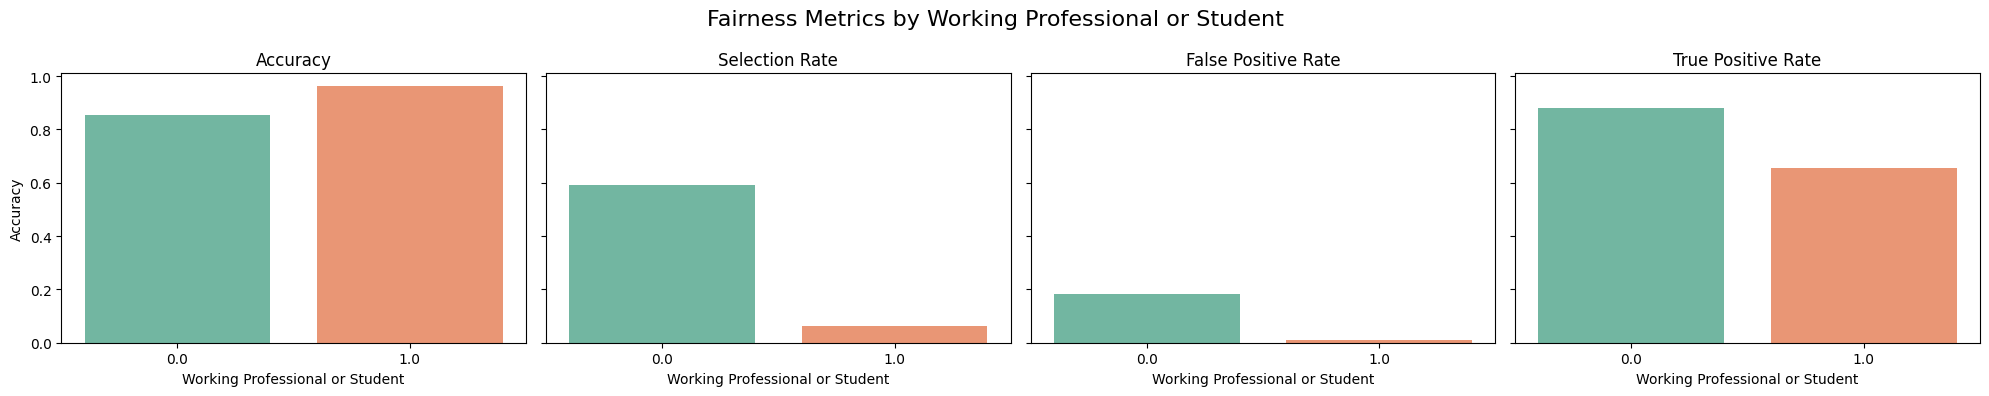
\includegraphics[width=\linewidth]{figures/mf_workingorstudent.png}
    \caption{Fairness metrics of the model, with Working Professional or Student as the sensitive feature.}
    \label{fig:mf_workingorstudent}
\end{figure}

These results suggest that, unlike with gender, the model's predictions vary meaningfully across employment status. This raises potential fairness concerns, particularly in how the model may be over-identifying depression among students while under-identifying it among working professionals. Given the real-world implications of such predictions in mental health interventions, these disparities warrant further investigation and potential mitigation.

To further explore the disparities observed between students and working professionals, we computed and visualized separate confusion matrices for each group. These plots, shown in Figure~\ref{fig:cm_workingorstudent}, provide a more detailed look at how the model behaves in terms of false positives, false negatives, and overall predictive performance for each subgroup.

\begin{figure}[h]
    \centering
    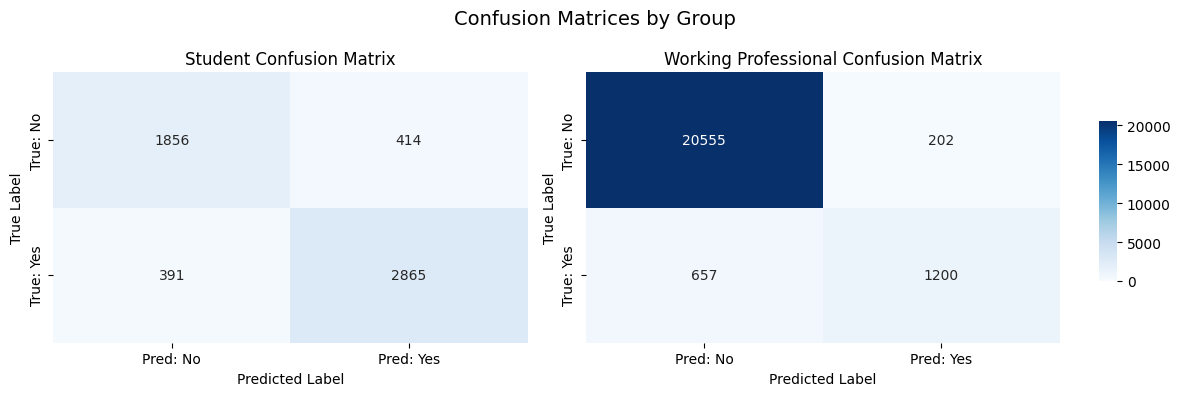
\includegraphics[width=\linewidth]{figures/cm.png}
    \caption{Group-specific confusion matrices with Working Professional or Student as the sensitive feature.}
    \label{fig:cm_workingorstudent}
\end{figure}

Specifically, working professionals not only had a notably higher accuracy ($\sim96\%$) than students ($\sim84\%$), but also higher FNR  ($\sim30\%$), indicating that depressive cases within this group were more likely to go undetected. Additionally, students experienced higher FPR ($\sim21\%$), meaning non-depressive individuals within this subgroup were more likely to be misclassified as depressive. 

In the student group (left panel), we observe a relatively balanced distribution of false positives and false negatives. While the model correctly identifies a large number of depressed students (2,865 true positives), it also generates a considerable number of false positives (414) and false negatives (391). This indicates that the model is relatively sensitive to depression in students, but it also errs in both directions.

By contrast, the confusion matrix for working professionals (right panel) reveals a different pattern. Here, the model shows a strong bias toward predicting the negative class: it identifies a large number of true negatives (20,555) and makes very few false positives (202). However, this comes at the cost of a much higher number of false negatives (657) and fewer true positives (1,200) compared to the student group.

Taken together, these results suggest that the model is more conservative in predicting depression among working professionals. It may be under-identifying true cases in this group, potentially due to differences in underlying feature distributions or label prevalence between students and working professionals. This finding complements the fairness metrics shown earlier and highlights a potential fairness concern: while the model performs well on average, it may systematically fail to detect depression in one group more than the other. This warrants further investigation, especially in high-stakes applications where underdiagnosis can have serious consequences.

To quantify the observed disparities between students and working professionals, we computed group-level disparity scores using a series of metrics provided by the \texttt{fairlearn.metrics} module. These metrics capture the absolute difference in model behavior across the two groups, using \texttt{Working Professional or Student} as the sensitive feature. The results are presented in Table~\ref{tab:ensemble_fairness}.

\begin{table}
\caption{Group-wise performance metrics for the L3 ensemble model using \texttt{Working Professional or Student} as the sensitive feature.}
\label{tab:ensemble_fairness}
\begin{tabular}{lrrrr}
\toprule
 & Accuracy & Selection Rate & True Positive Rate & False Positive Rate \\
\midrule
\textbf{Student (0)} & 0.854300 & 0.603900 & 0.888800 & 0.195200 \\
\textbf{Working Professional (1)} & 0.962000 & 0.062800 & 0.651100 & 0.010200 \\
\bottomrule
\end{tabular}
\end{table}

As shown in the table, the most pronounced disparity appears in the selection rate, with a difference of 0.5314 between groups. This indicates that one group is far more likely to be predicted as positive than the other. Substantial differences are also observed in the true positive rate (0.2337) and false positive rate (0.1726), suggesting that the model’s sensitivity and error patterns vary meaningfully across groups. Even the accuracy difference, which is typically more stable across subpopulations, exceeds 10\%, underscoring that the model’s predictive performance is not uniform between students and working professionals.

Together, these metrics provide strong evidence of group-level disparities in how the model assigns predictions. The magnitude of these differences suggests that additional investigation and potentially mitigation are warranted, especially in applications where equity in prediction outcomes is critical.
 

Again to emphasize, when model was retrained and validated separately for professionals and students (with dropping non-relevant features), these high values of FNR and FPR respectively were maintained (~\ref{fig:orig_vs_stu}). This suggests that the \textit{data} and not just the model architecture drives this disparity. This may be due to the reasons like: (i) Student responses may be more inconsistent or self-reported (and for professionals they might come from clinical diagnoses), leading to noisy ground truth, making the model learn unreliable patterns, causing unstable FPR/FNR tradeoff. Figure~\ref{fig:dep_count_stu} indicates that since ground truth depression for students is much higher than \texttt{Not Depressed}, and even 7-fold higher than Depressed professionals, the model might have overfit, and led to poor generalization. 

\begin{figure}[H]
    \begin{minipage}{0.45\textwidth}
        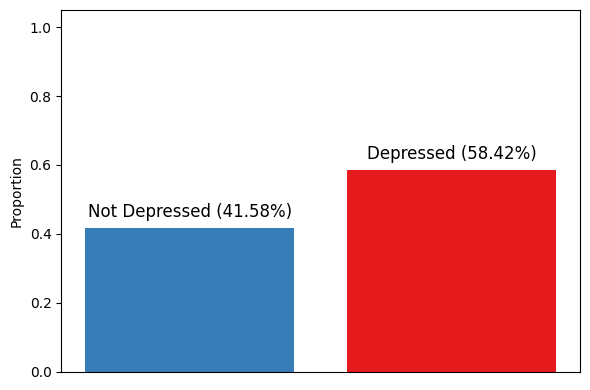
\includegraphics[width=\linewidth]{figures/dep_count_stu.png} 
        \caption{True Counts in Training Data (Students)}
    \label{fig:dep_count_stu}
    \end{minipage}
    \hfill
   \begin{minipage}{0.45\textwidth}
        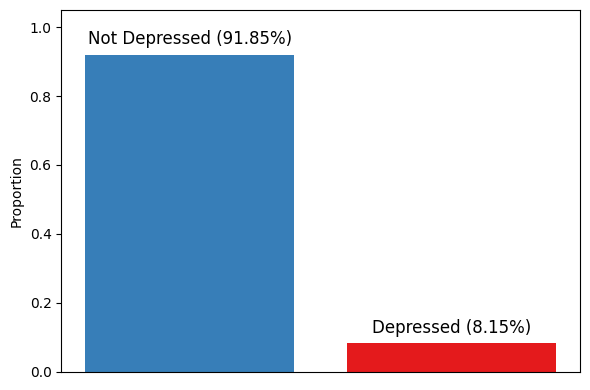
\includegraphics[width=\linewidth]{figures/dep_count_prof.png} 
        \caption{True Counts in Training Data (Working Professionals)}
    \end{minipage}
    \label{fig:dep_count_prof}
\end{figure}

\begin{figure}[H]
    \centering
    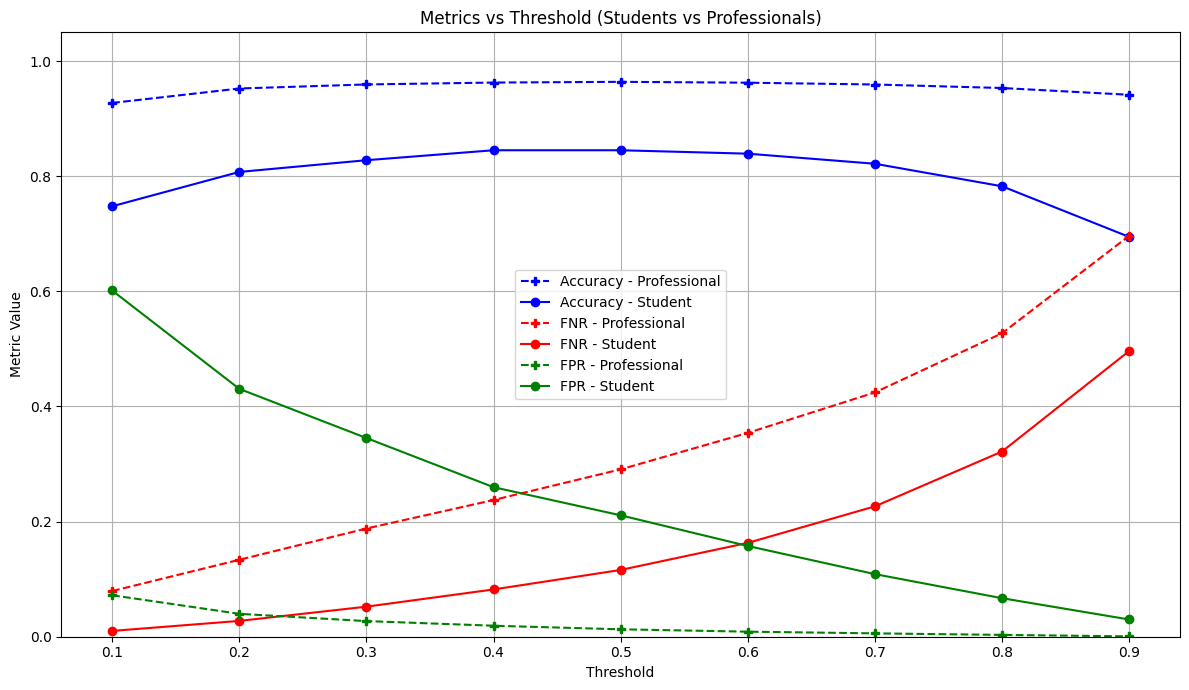
\includegraphics[width=0.7\linewidth]{figures/threshold.png}
    \caption{How metrics change with Classification Threshold}
    \label{fig:threshold}
\end{figure}
(ii) Additionally, the decision threshold (probability less than 0.5 is classified 0, and more than 0.5 is 1) is neither optimized nor group-specific. The same threshold might cause under-detection in professionals (hence high false negative rate) and over-detection in students (high false positive rate). This suggests that overall and group-specific calibration might be necessary. Figure~\ref{fig:threshold} clearly indicates the significant gap in accuracy, FNR, and FPR values between students (bold lines) and working professionals (dotted lines). Though the threshold 0.5 optimizes the gap in accuracy, it doesn't balance the fairness needs of the model. However, an important observation is that even when threshold is modified, there is not much change in accuracy for both the groups, but there can be significant changes in fairness performances, if threshold is optimized. For example, as the threshold increases, false positive rate difference decreases with coming close to 0 at threshold 0.9. 


In acccordance with above observations and to address the fairness disparities observed across employment groups, we applied \texttt{Fairlearn}’s \texttt{ThresholdOptimizer}, a post-processing mitigation technique designed to enforce fairness constraints without retraining the underlying model. In our case, we selected the \texttt{equalized\_odds} constraint, which seeks to equalize both true positive and false positive rates across groups. This choice was motivated by our prior audit, which revealed substantial disparities in sensitivity and error rates between students and working professionals.

Table~\ref{tab:ensemble_fairness_equalized_odds} reports the group-wise performance metrics after threshold optimization. While overall accuracy decreases for the student group, the true positive rates for both groups become closely aligned (0.5992 for students vs. 0.5918 for working professionals), and false positive rates converge as well (0.0370 vs. 0.0385). These results suggest that threshold optimization effectively reduces disparity in model behavior across groups, trading off a modest reduction in predictive performance for improved fairness in classification outcomes.

\begin{table}[H]
\caption{Post-mitigation fairness metrics for the L3 ensemble using \texttt{Working Professional or Student} as the sensitive feature, optimized for equalized odds.}
\label{tab:ensemble_fairness_equalized_odds}
\begin{tabular}{lrrrr}
\toprule
& Accuracy & Selection Rate & True Positive Rate & False Positive Rate \\
\midrule
\textbf{Student (0)} & 0.748600 & 0.368300 & 0.599200 & 0.037000 \\
\textbf{Working Professional (1)} & 0.931100 & 0.084000 & 0.591800 & 0.038500 \\
\bottomrule
\end{tabular}
\end{table}

\begin{figure}[H]
\centering
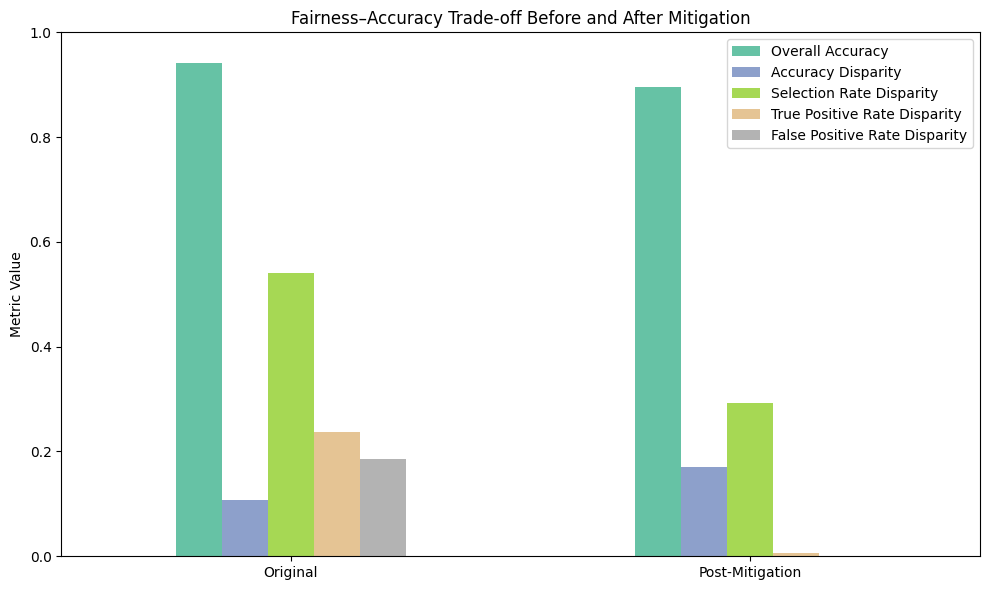
\includegraphics[width=0.6\linewidth]{figures/fairness_tradeoff.png}
\caption{Fairness–accuracy trade-off before and after applying threshold optimization for equalized odds.}
\label{fig:fairness_tradeoff}
\end{figure}
To visualize this trade-off, we compare the original ensemble model and the mitigated version across key fairness and accuracy metrics. As shown in Figure~\ref{fig:fairness_tradeoff}, threshold optimization leads to a small reduction in overall accuracy (from 94\% to 90\%) but results in substantial improvements in fairness: disparities in true and false positive rates nearly vanish, and selection rate disparity decreases by over 40 percentage points. These shifts illustrate the practical cost of enforcing group fairness and highlight the importance of balancing equity and performance in sensitive applications like mental health screening.




\section{Prediction Interpretation}
To better understand how our ensemble model makes predictions—and whether those decisions align with human expectations—we applied LIME (Local Interpretable Model-Agnostic Explanations) \parencite{ribeiro2016why}. LIME explains individual predictions by locally approximating the model with an interpretable surrogate, such as a linear model. However, our final L3 ensemble combines two second-level learners: \texttt{l2-ensemble-lr} (logistic regression) and \texttt{l2-ensemble-ridge} (ridge regression), using a weighted average of their predicted probabilities. While logistic regression exposes the \texttt{predict\_proba} interface needed for LIME, ridge regression does not natively provide probabilistic outputs. Consequently, for interpretability purposes, we restricted LIME analysis to the logistic regression component of the ensemble.

This choice introduces an important caveat: as shown in Figure~\ref{fig:l3_weights}, the final ensemble assigns only \textbf{1.4\%} of the total weight to the logistic regression model, while the ridge regression component dominates with 98.6\%. Therefore, while LIME offers useful intuition into local feature contributions under a linear model, the resulting explanations must be interpreted with caution. They reflect the behavior of a minor contributor to the ensemble, and thus do not fully represent the decision logic of the final model.

\begin{figure}[h]
\centering
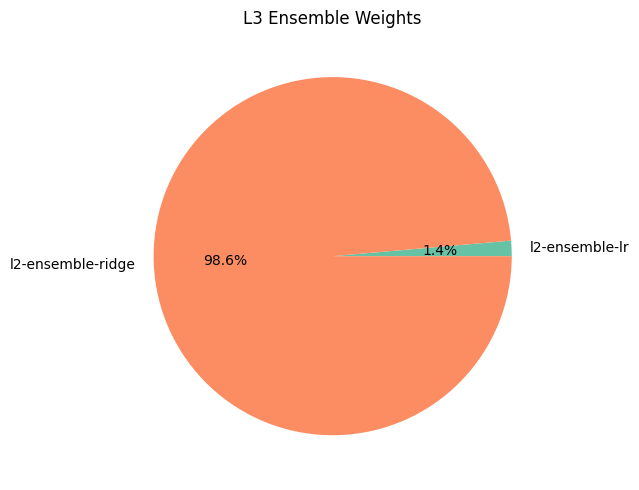
\includegraphics[width=0.4\linewidth]{figures/l2_weights.png}
\caption{L3 ensemble weights assigned to the second-level models. The final prediction is heavily dominated by \texttt{l2-ensemble-ridge}.}
\label{fig:l3_weights}
\end{figure}

Despite this limitation, LIME still provides a transparent lens into how one interpretable component processes the data, and allows us to inspect patterns of misclassification and borderline decisions in a structured way.

We used LIME to analyze three representative validation cases: a misclassified working professional, a misclassified student, and an uncertain but correct prediction. These examples were selected to probe potential group-specific failure modes and examine the model’s behavior near the decision boundary.

\begin{figure}[H]
\centering
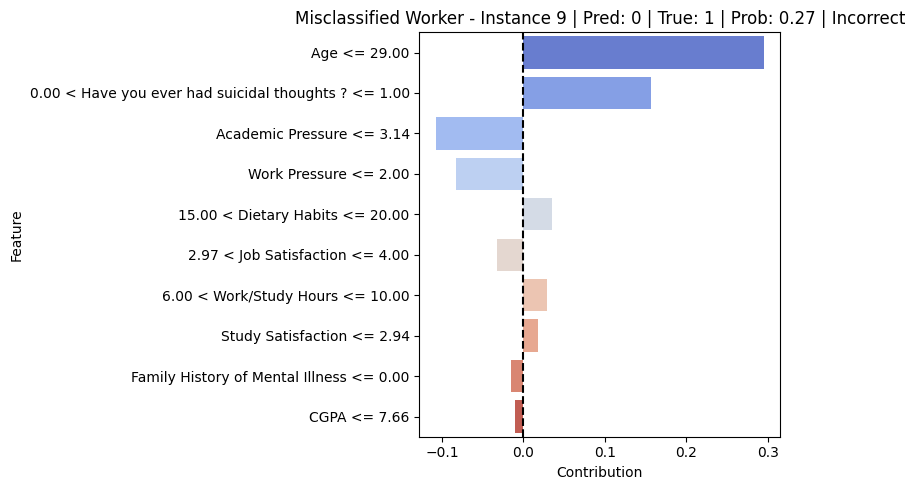
\includegraphics[width=0.9\linewidth]{figures/lime_mis_prof.png}
\caption{LIME explanation for a misclassified working professional (true: depressed, predicted: not depressed). Blue bars indicate features contributing to the negative class (“No”), red bars indicate features contributing to the positive class (“Yes”).}
\label{fig:lime_mis_prof}
\end{figure}

In the first example~\ref{fig:lime_mis_prof}, a working professional was incorrectly classified as not depressed despite self-reporting suicidal ideation and experiencing work pressure. The predicted probability was just 27\%. LIME revealed that older age and low work pressure were dominant negative contributors, outweighing more concerning signals. This case illustrates how the model may be biased toward under-identifying depression among working professionals when protective features are present, even alongside serious risk indicators.


In the second case~\ref{fig:lime_mis_student}, a student was incorrectly classified as depressed, with a predicted probability of 64\%. While this individual showed low financial stress and no family history of mental illness, the model was strongly influenced by age, suicidal ideation, and academic pressure, factors it learned to associate with depression in younger populations. Although understandable, this case demonstrates how the model may over-identify depression among students, consistent with the earlier finding of selection rate disparity by employment group.

\begin{figure}[h]
\centering
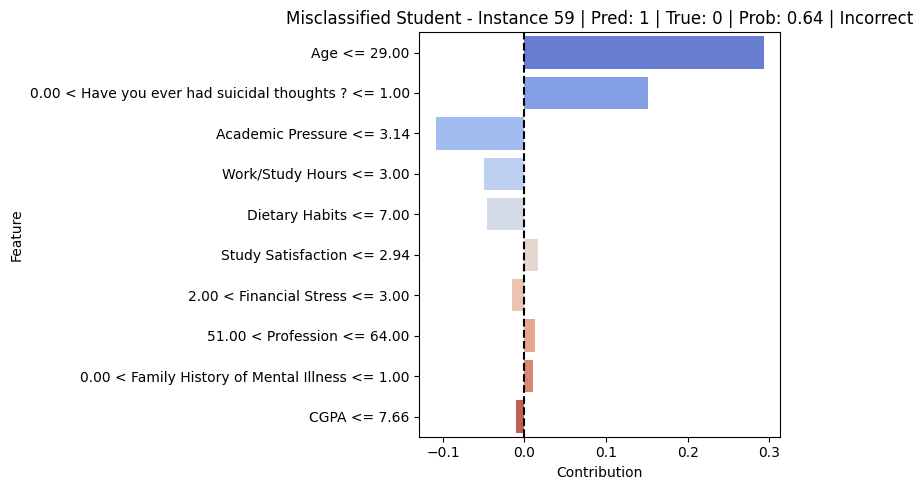
\includegraphics[width=0.8\linewidth]{figures/lime_mis_student.png}
\caption{LIME explanation for a misclassified student (true: not depressed, predicted: depressed).}
\label{fig:lime_mis_student}
\end{figure}

Lastly~\ref{fig:lime_uncertain}, we examined a borderline case with a correct prediction. Here, the model output a probability of 50\% for depression, ultimately predicting the correct label. No single feature dominated the explanation; instead, moderate academic pressure and financial stress were offset by the absence of suicidal thoughts. This example highlights the model’s capacity to handle ambiguity by balancing weak signals, an encouraging sign, though such behavior may also be fragile.

\begin{figure}[h]
\centering
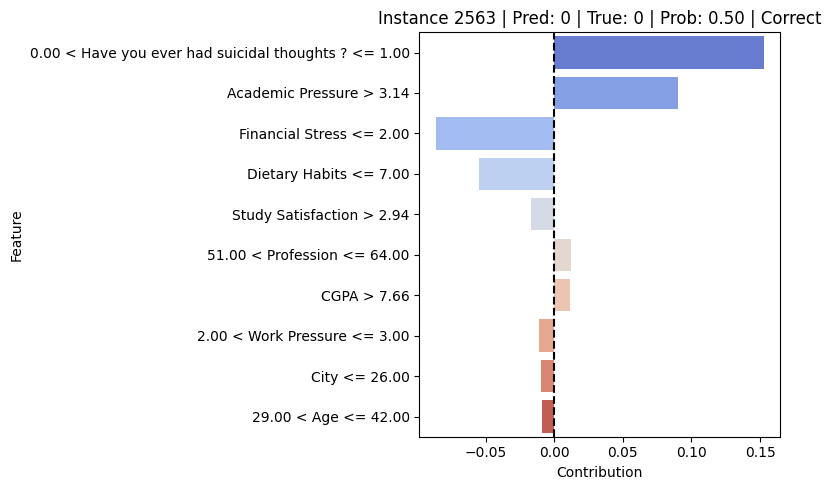
\includegraphics[width=0.75\linewidth]{figures/lime_uncertain.png}
\caption{LIME explanation for a correct but uncertain prediction (true: not depressed, predicted: not depressed, probability: 50\%).}
\label{fig:lime_uncertain}
\end{figure}

These local explanations lend transparency to model behavior, reinforce the fairness concerns raised earlier, and offer valuable guidance for future model debugging and refinement.


\typeout{}
\chapter{Conclusion}

While the model audited in this project demonstrates strong predictive accuracy, we find that the underlying dataset poses significant challenges for responsible deployment in an automated decision system (ADS). The data is synthetically generated with unclear provenance and shows substantial geographic and demographic biases, particularly overrepresentation of urban centers in North and Central-West India and underrepresentation of rural, southern, and northeastern regions. Moreover, culturally relevant variables such as family structure, interpersonal relationships, and stigma-related experiences, which are central to understanding depression in the Indian context, are missing. As a result, while the dataset is useful for experimentation and benchmarking, it is not appropriate for real-world, fairness-sensitive applications without considerable expansion and refinement.

The implementation itself is robust in terms of accuracy, with the final ensemble achieving over 94\% on held-out validation data. However, fairness evaluations tell a different story. While gender-based disparities were minimal, significant disparities emerged along employment status: students were over-identified as depressed (high false positive rate), while working professionals were often missed (high false negative rate). These findings were confirmed through \texttt{MetricFrame} audits, confusion matrices, and local explanations using \texttt{LIME}. To address these disparities, we applied \texttt{Fairlearn}’s \texttt{ThresholdOptimizer} with an equalized odds constraint. This post-processing method successfully reduced group-level disparities in true and false positive rates, at the cost of a modest drop in accuracy ($\sim 4\%$). Given the sensitive nature of mental health prediction, we believe this is an acceptable trade-off. Stakeholders such as clinicians, patients, and policy makers would likely find fairness metrics, particularly false negative and false positive rates, more meaningful than accuracy alone, as these capture the real-world harms of misclassification.

Despite improvements, we would not recommend deploying this model in the public sector or industry in its current form. The lack of transparency in data sourcing, insufficient cultural representation, and observed subgroup disparities make it unsuitable for high-stakes decision-making without further development. Future iterations should incorporate richer, more representative data; include culturally and socially relevant features; apply fairness interventions during model training rather than solely post hoc; and calibrate prediction outputs to support informed threshold selection. Only with these enhancements can such a model be responsibly used to support equitable and trustworthy mental health screening at scale.
% \typeout{}
\chapter*{\centering Acknowledgements}
\quad We would like to acknowledge our teaching assistant, Manasvin Anand, for his valuable guidance, prompt feedback, and continuous support throughout this audit project. His insights were instrumental in helping us navigate both technical challenges and conceptual clarity during our work.


\printbibliography
\typeout{}

\appendix
\chapter{Data Distribution}
\label{appendix}
(Referring to the \parencite{GoogleDriveI/O})

The data is synthetically generated by a deep learning model. The data is distributed similarly to the original data that the model was trained on \parencite{ravaghiS04E11MentalHealth2024}.

\resizebox{\textwidth}{!}{ 
\begin{tabular}{|c|c|c|l|}
\hline
 Col\#&  Column name &  datatype&  Feature values\\ 
 \hline
0 & id & int64 &  [0, 1, 2, 3, 4, 5, ...\\ \hline
 1& Name & object & [Aaradhya, Vivan, Yuvraj, ... \\ \hline
 2& Gender & object & [Female, Male] \\ \hline
3 & Age & float64 & [49.0, 26.0, 33.0, ... \\ \hline
4 & City  & object &  [Ludhiana, Varanasi, Visakhapatnam, ...\\ \hline
5 & Working Professional or Student & object & [Working Professional, Student] \\ \hline
6 & Profession & object &  [Chef, Teacher, nan, Business Analyst, ...\\ \hline
7 & Academic Pressure & float64 & [5.0, 4.0, 3.0, 2.0, 1.0] \\ \hline
8 & Work Pressure & float64  &  [5.0, 4.0, 3.0, 2.0, 1.0]\\ \hline
9 & CGPA & float64 & [0-10]  \\ \hline
10 & Study Satisfaction & float64 &  [5.0, 4.0, 3.0, 2.0, 1.0]\\ \hline
11 & Job Satisfaction  & float64 & [5.0, 4.0, 3.0, 2.0, 1.0] \\ \hline
12 & Sleep Duration & object &  [More than 8 hours, Less than 5 hours, 5-6 hours, ...\\ \hline
13 & Dietary Habits & object &  [Healthy, Unhealthy, Moderate, ...\\ \hline
14 & Degree & object & [BHM, LLB, B.Pharm, BBA,... \\ \hline
15 & Have you ever had suicidal thoughts ? &  object &  [No, Yes]\\ \hline
16 & Work/Study Hours & float64  & [1.0, 2.0, ..., 11.0] \\ \hline
17 & Financial Stress & float64 & [5.0, 4.0, 3.0, 2.0, 1.0] \\ \hline
18 & Family History of Mental Illness & object & [No, Yes] \\ \hline
\rowcolor{yellow}
19 & (Target Value) Depression & int64 & [0, 1] \\\hline
\end{tabular}
}

\section{Null Values}

The dataset contains significant missing values for several attributes, including `Profession', `Academic Pressure', `Work Pressure', `CGPA', `Study Satisfaction', `Job Satisfaction', `Dietary Habits', `Degree', and `Financial Stress'.

The missing values can be understood as follows. Students often leave fields such as `Profession', `Work Pressure', and `Job Satisfaction' blank because these attributes are not relevant to their situation, or, in some cases, individuals may not feel comfortable sharing details about their jobs. On the other hand, working professionals tend to omit values for `Academic Pressure', `CGPA', and `Study Satisfaction', as these fields are similarly irrelevant to them.

Other attributes might simply be missing due to the synthetic data generation process. Else, in the case of missing values for `Degree' (two rows), both individuals were identified as working professionals who also chose not to specify their professions. This may suggest discomfort in disclosing qualifications.

The missing values for `Dietary Habits' and `Financial Stress' (four rows each), however, remain unexplained. These omissions do not appear to follow a clear pattern.

\section{Data Analysis} 

As part of the exploratory data analysis (EDA), we plotted the distribution of all features, as well as all features by gender (sensitive attribute) and depression (target). Considering the large number of plots, we only included figures that are essential or surprising in relation to this project in this report. All figures can be found in the Google Colab Notebook. \\

\begin{figure}[H]
    \centering
    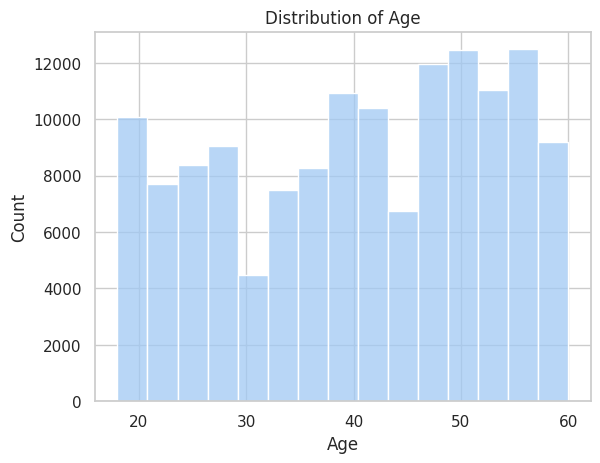
\includegraphics[width=0.5\textwidth]{edafigures/age_dist.png}
    \caption{Distribution of age of the participants.}
    \label{fig:age_dist}
\end{figure}

\noindent Figure~\ref{fig:age_dist} is the general distribution of age of the sample. As you can see, the distribution is approximately uniform, with slightly more older than younger adults.\\

Figure~\ref{fig:gender_dist} is the distribution of gender of the sample. As you can see, there are more males than females in this sample.\\
\begin{figure}[H]
    \centering
    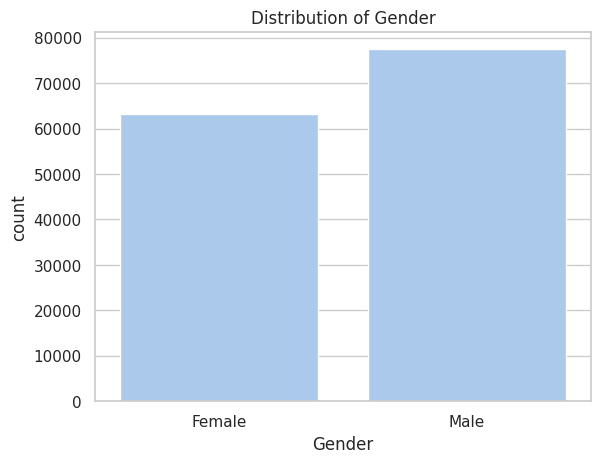
\includegraphics[width=0.5\textwidth]{edafigures/gender_dist.png}
    \caption{Distribution of gender of the participants.}
    \label{fig:gender_dist}
\end{figure}
Similarly, the distribution of depression is presented as figure~\ref{fig:dep_dist}. Not surprisingly, the rate of depression is relatively low, which is consistent with our expectation. However, the prevalence of depressed individuals in this sample is 18.2\%, which is way higher than the population average. Considering the data is synthetically generated with the purpose of depression detection, the depression prevalence can be explained. 

\begin{figure}[H]
    \centering
    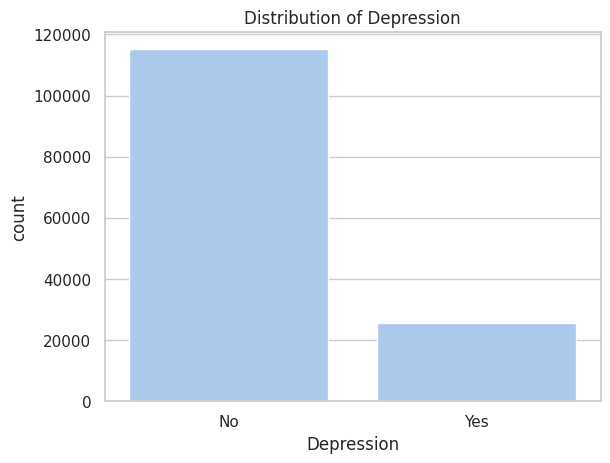
\includegraphics[width=0.5\textwidth]{edafigures/dep_dist.png}
    \caption{Distribution of depression.}
    \label{fig:dep_dist}
\end{figure}

To get a basic sense of how depression distributes relative to our sensitive attribute, gender, we plotted depression by gender. The resulting figure is figure~\ref{fig:dep_gender}. Contrary to our expectation and general consensus \parencite{APA2013DSM5}, there are slightly more depressed males than there are females. One potential explanation is that the data is simulating features of Indian population, which could have a different gender prevalence when it comes to depression than the one based on almost completely U.S. and Western context. \\

\begin{figure}[H]
    \centering
    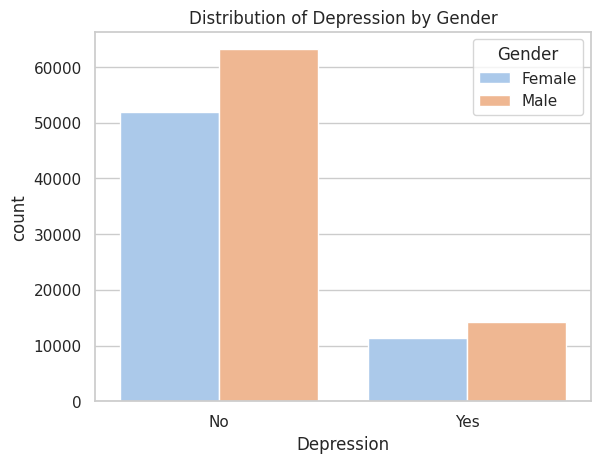
\includegraphics[width=0.6\linewidth]{edafigures/dep_gender.png}
    \caption{Depression by Gender.}
    \label{fig:dep_gender}
\end{figure}

Another interesting aspect of this dataset we discovered through EDA is the distribution of age in terms of depression. See figure~\ref{fig:age_dep}. The mean age of depressed individuals is substantially lower than that of the not depressed ones, at around 23 years of age, while the mean age of not depressed participants is around 35. The age distribution aligns with published studies on the age of onset of depression \parencite{mirowskyAgeDepression1992}, where there is a large spike in depression rate for people between the ages of 17 and 25, and again for people that are over 80 years of age. Though there are more working professionals than students in this dataset (results not shown), there is a much higher rate of depression in young adults. This trend indicates a possibility of treating age as a sensitive attribute, as it might lead to imbalanced model prediction based on age alone. To explore this possibility, we calculated the point-biserial correlation of age and depression, which we will present and report in the later sections. 
\begin{figure}[H]
    \centering
    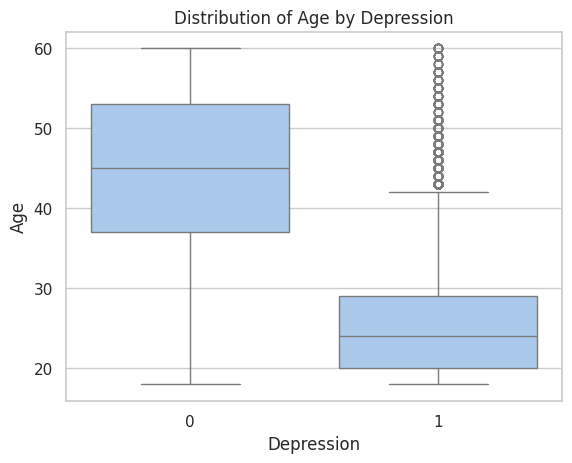
\includegraphics[width=0.6\linewidth]{edafigures/age_dep.png}
    \caption{Distribution of age by depression.}
    \label{fig:age_dep}
\end{figure}

\begin{figure}[H]
    \centering
    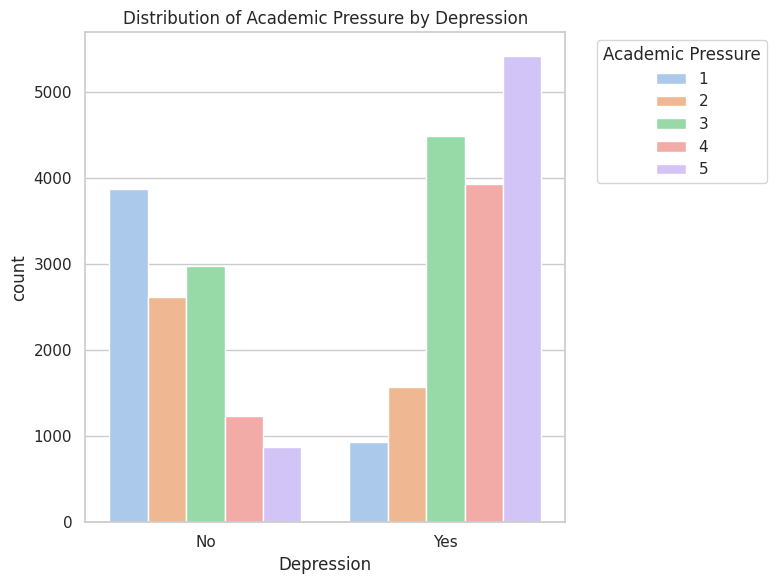
\includegraphics[width=0.6\linewidth]{edafigures/academicPressure_dep.png}
    \caption{Distribution of academic pressure and depression.}
    \label{fig:academicPressure_dep}
\end{figure}

Figure~\ref{fig:academicPressure_dep} illustrates the relationship between academic pressure and depression. The distribution for non-depressed individual is clearly negatively skewed, while the distribution for depressed individual is the direct opposite. This result makes intuitive sense, as one would expect the perceived stress would have a relationship with depression. Similar trends are observed in the relationship between work pressure and depression, and opposite trends are observed in the relationship between study satisfaction and job satisfaction and depression, in the sense that depressed individuals reported less satisfaction in their study or job than non-depressed individuals.

% \newpage
\subsection{Feature Correlation}\label{feature_corr}

As illustrated in Figure~\ref{fig:age_dep}, the sigmoid curve depicted in Figure~\ref{fig:prob_age_depression} clearly demonstrates that the probability of depression is higher among young adults. This can be attributed to the fact that students exhibit significantly higher rates of depression compared to working professionals (Figure~\ref{fig:depression_empoyment}). Furthermore, the correlation matrix shown in Figure~\ref{fig:corr_depression} emphasizes that attributes such as unhealthy dietary habits, inadequate sleep duration, and the occurrence of suicidal thoughts are positively correlated with each other and are notably associated with students. 

\begin{figure}[H]
    \centering
    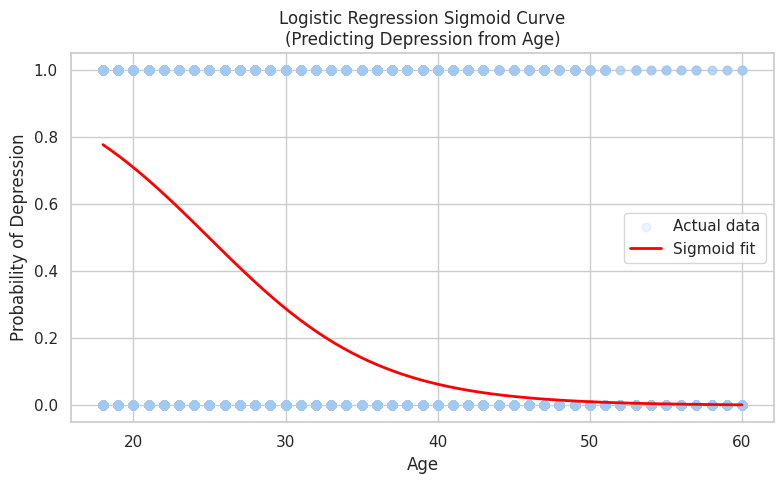
\includegraphics[width=0.5\linewidth]{edafigures/prob_age_depression.png}
    \caption{Predicting Depression from Age}
    \label{fig:prob_age_depression}
\end{figure}

\begin{figure}[H]
    \centering
    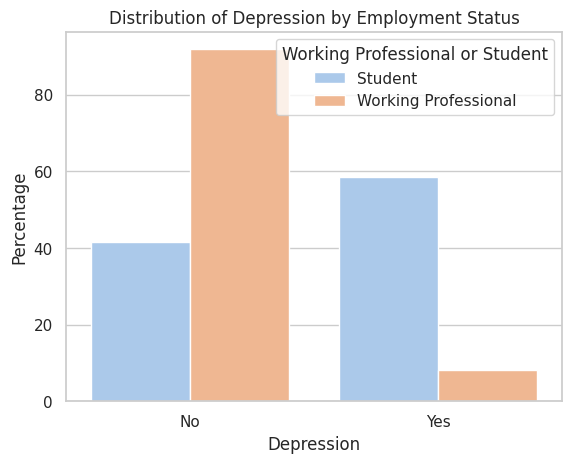
\includegraphics[width=0.5\linewidth]{edafigures/depression_empoyment.png}
    \caption{Distribution of Employment Status vs Depression}
    \label{fig:depression_empoyment}
    
\end{figure}

\begin{figure}[H]
    \begin{minipage}{0.5\textwidth}
        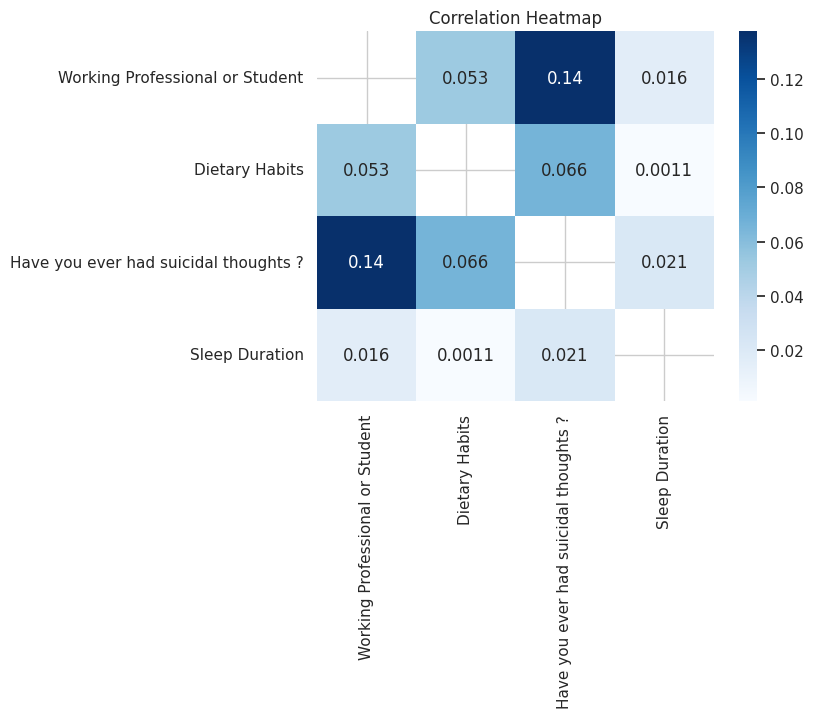
\includegraphics[width=\linewidth]{edafigures/corr_depression.png} 
        \caption{Correlation of Employment Status, Dietary Habits, Sleep Duration and Suicidal Thoughts.}
    \label{fig:corr_depression}
    \end{minipage}
    \hfill
    \begin{minipage}{0.45\textwidth}
        \scriptsize{
        Student:1, Working Professional:0\\
        Unhealthy: 2, Moderate: 1, Healthy:0\\
        Sleep : $<$ 5 hours:3, 5-6 hours:2, $>$ 8 hours: 1, 7-8 hours: 0\\
        Suicidal Thoughts: Yes: 1, No: 0}
    \end{minipage}
\end{figure}

Our analysis as shown in Figure~\ref{fig:corr_gender_work} also reveals a positive correlation between gender (-1 for males, 1 for females) and work pressure, consistent with prior studies indicating women face higher work pressure due to overlapping professional and caregiving roles, especially during remote work setups \parencite{rabuni2023worklifebalance}.

\begin{figure}[H]
    \centering
    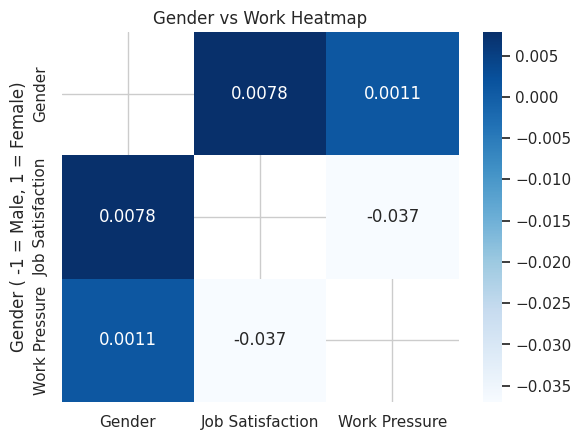
\includegraphics[width=0.5\linewidth]{edafigures/corr_gender_work.png}
    \caption{Distribution of Gender vs Work Pressure and Job Satisfaction}
    \label{fig:corr_gender_work}
\end{figure}

Interestingly, the data also indicates a positive correlation between gender and job satisfaction. This observation appears to contradict prior studies that associate lower job satisfaction among women with discriminatory organizational practices and societal expectations \parencite{karthikkumar2024worklifebalanc}. One potential explanation for this contradiction might lie in the study's context—data was collected from selected urban cities in India, where unique factors could influence these findings. For instance, exceptions in prior research suggest that variables such as locus of control can sometimes neutralize gender disparities in job satisfaction \parencite{talamala2024locuscontrol}.


Another aspect of the data distribution is shown in Figure~\ref{fig:regionwise} and~\ref{fig:regional_distri} , which suggests that dataset primarily includes data from major cities in larger states of India, predominantly from the Central North and Central-West regions. This lack of data from small-to-medium cities, rural areas, and regions like the South, Central-East, and North-East India might be an unrepresentative sample.
\begin{figure}[H]
    \centering
    \begin{minipage}{0.45\textwidth}
        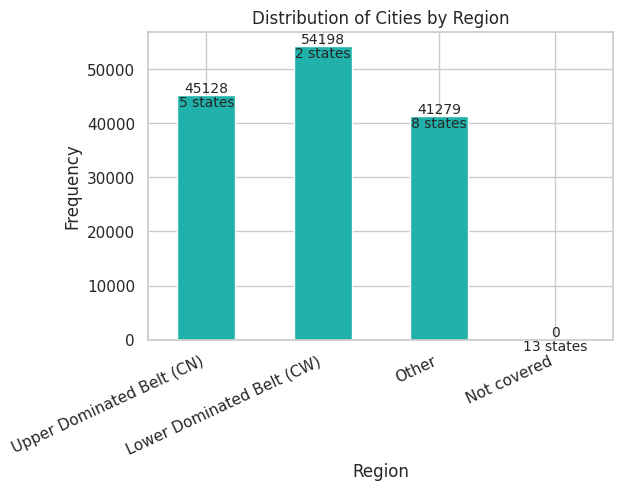
\includegraphics[width=\linewidth]{edafigures/regionwise.png}
        \caption{Data Distribution Region-wise}
        \label{fig:regionwise}
    \end{minipage}
    \hfill
    \begin{minipage}{0.45\textwidth}
        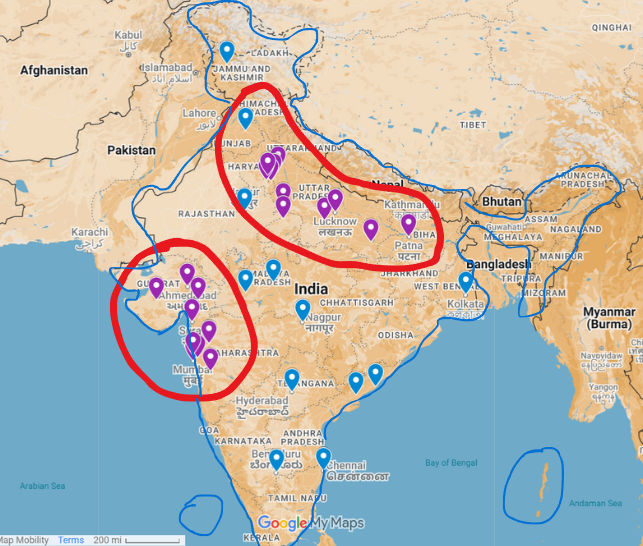
\includegraphics[width=\linewidth]{edafigures/regional_distri.png}
        \caption{Map Annotation of Training Data, depicting biased selection}
        \label{fig:regional_distri}
    \end{minipage}
\end{figure}

\section{Post Training Analysis}\label{post_train}

\begin{figure}[h]
    \centering
    
\includegraphics[width=0.6\linewidth]{figures/regionwise.png}
    \caption{Overall Performance w.r.t. Region After Model Training}
    \label{fig:region_overall}
\end{figure}

\begin{figure}[H]
    \centering
    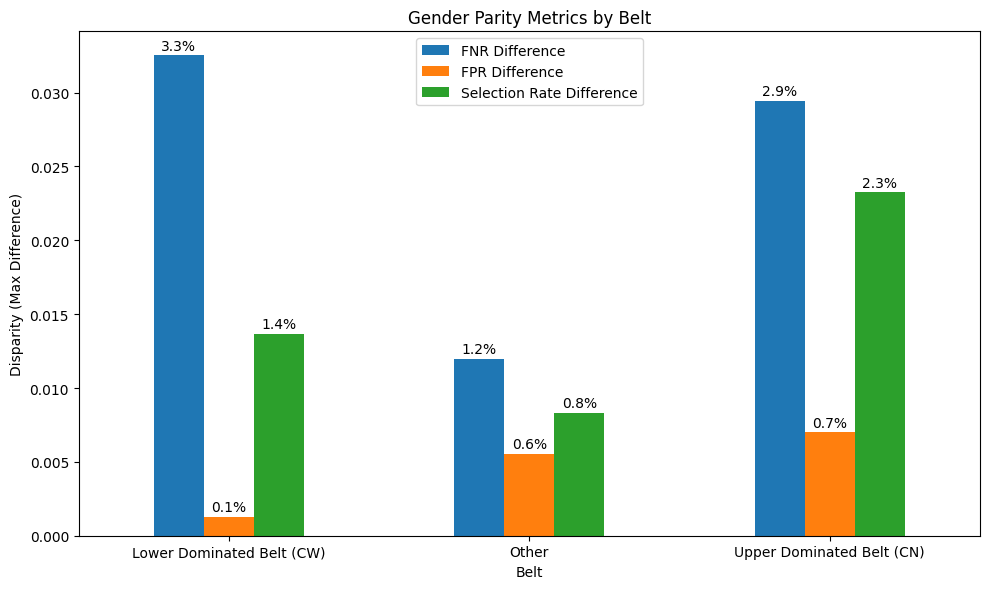
\includegraphics[width=0.6\linewidth]{figures/region_parity.png}
    \caption{Fairness w.r.t. Gender for Region After Model Training}
    \label{fig:region_gender}
\end{figure}

\begin{figure}[H]
    \centering
    \begin{minipage}{0.48\textwidth}
            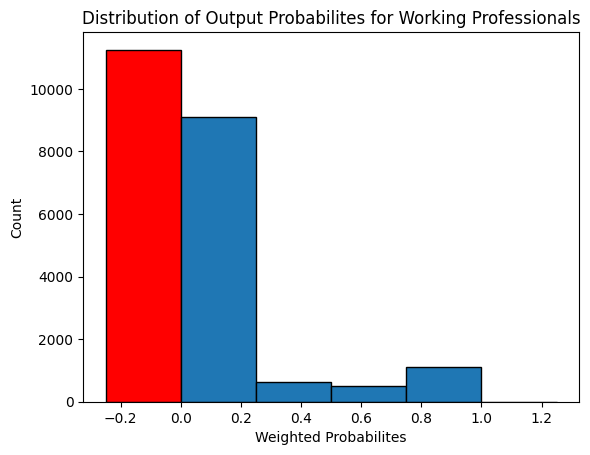
\includegraphics[width=\linewidth]{figures/prob_distri_prof.png}
    \end{minipage}
    \hfill
    \begin{minipage}{0.48\textwidth}
         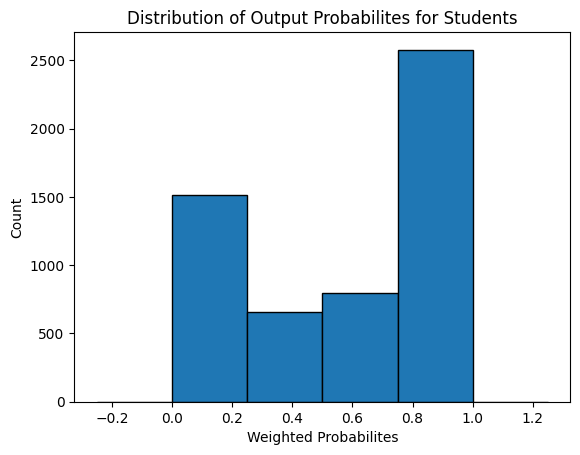
\includegraphics[width=\linewidth]{figures/prob_distri_stu.png}
    \end{minipage}
    \caption{The output ``probabilites" for Working Professionals are outside the range of [0,1], with a significant count in less than 0, which cannot be ignored or considered outliers. This imply that there is an in-processing need for scaling such distribution, as they don't clearly justify the predicted outcome. This also strengthens the argument for optimizing threshold for classification.}
    \label{fig:prob_distri}
\end{figure}




\end{document}
